\documentclass{article}
\usepackage{geometry}
\usepackage{graphicx}


\title{Pràctica 3 Llenguatge de Marques}
\author{Francesc Mut Mollà}

\begin{document}
\maketitle
\newpage
\section{Exercici 1}

\begin{verbatim}
<?xml version="1.0" encoding="UTF-8"?>

<!DOCTYPE missatges [
<!ELEMENT missatges (missatge)>
<!ELEMENT missatge (telefono, fecha, hora, titol_missatge,cos_missatge)>
<!ELEMENT telefono (#PCDATA)>
<!ELEMENT fecha (#PCDATA)>
<!ELEMENT hora (#PCDATA)>
<!ELEMENT titol_missatge (#PCDATA)>
<!ELEMENT cos_missatge (#PCDATA)>
]>
<missatges>
    <missatge>
        <telefono>123124125</telefono>
        <fecha>30-04-21</fecha>
        <hora>19:04:30</hora>
        <titol_missatge>Lorem Ipsum</titol_missatge>
        <cos_missatge>Dolor sit amet</cos_missatge>
    </missatge>
</missatges>
\end{verbatim}
\vspace{3cm}
\begin{center}
\textit{Comprovant de validació.}
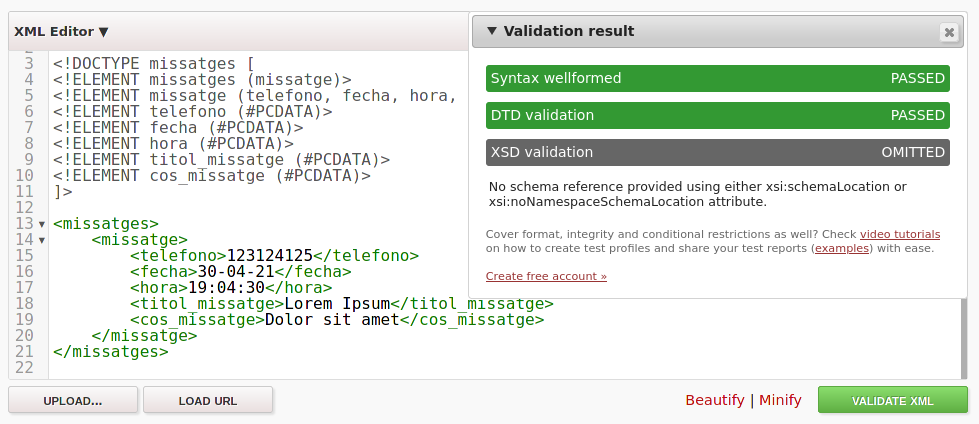
\includegraphics[width=12cm]{validacio1.png}
\end{center}

\newpage


\section{Exercici 2}

\begin{verbatim}
<?xml version="1.0" encoding="UTF-8"?>

<!DOCTYPE biblioteca [
  <!ELEMENT biblioteca (llibre*)>
  <!ELEMENT llibre (titol, editorial, (edicio | ISBN), numero_de_pagines?, autor*)>
  <!ELEMENT titol (#PCDATA)>
  <!ELEMENT editorial (#PCDATA)>
  <!ELEMENT edicio (#PCDATA)>
  <!ELEMENT ISBN (#PCDATA)>
  <!ELEMENT numero_de_pagines (#PCDATA)>
  <!ELEMENT autor (#PCDATA)>
  <!ATTLIST llibre codi ID #REQUIRED>
]>
<biblioteca>
<llibre codi="id1">
    <titol>No me cuentes tu vida</titol>
    <editorial>Planeta</editorial>
    <ISBN>9788408013877</ISBN>
    <numero_de_pagines>464</numero_de_pagines>
    <autor>Luis García Montero</autor>
</llibre>
<llibre codi="id2">
    <titol>Física para la Ciencia y Tecnología</titol>
    <editorial>Reverte</editorial>
    <edicio>Primera edició</edicio>
    <numero_de_pagines>702</numero_de_pagines>
    <autor>Paul A. Tipler</autor>
</llibre>
</biblioteca>
\end{verbatim}
\vspace{0,5cm}
\begin{center}
    \textit{Comprovant de validació.}
    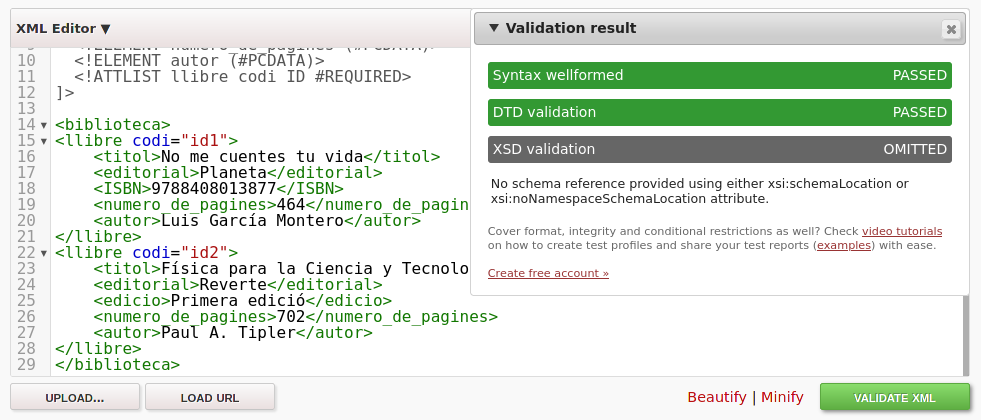
\includegraphics[width=12cm]{validacio2.png}
\end{center}
    
\newpage

\section{Exercici 3}

\begin{verbatim}
<?xml version="1.0" encoding="UTF-8"?>

<!DOCTYPE llistaCompra [
<!ELEMENT llistaCompra (producte*)> <!--Faltava un >-->
<!ELEMENT producte (quantitat, nom, preu)>
<!ATTLIST producte ref CDATA #REQUIRED>
<!ATTLIST producte fecha CDATA #IMPLIED> 
<!ATTLIST producte seccio (alimentacio | drogueria | congelats) #REQUIRED>
<!ELEMENT nom (#PCDATA)> <!--Afegit element nom-->
<!ELEMENT quantitat (#PCDATA)>
<!ELEMENT preu (#PCDATA)>
]>
<llistaCompra>
    <producte ref="1321" fecha="30-04-21" seccio="alimentacio">
        <quantitat>15</quantitat>
        <nom>Pepinos</nom>
        <preu>3,30€</preu>
    </producte>
    <producte ref="5141" fecha="30-04-21" seccio="drogueria">
        <quantitat>32</quantitat>
        <nom>Aiguarrás</nom>
        <preu>3,93</preu>
    </producte>
    <producte ref="1231" fecha="30-04-21" seccio="congelats">
        <quantitat>12</quantitat>
        <nom>Calamars</nom>
        <preu>5,70</preu>
    </producte>
</llistaCompra>
\end{verbatim}
\vspace{,5cm}
\begin{center}
    \textit{Comprovant de validació.}
    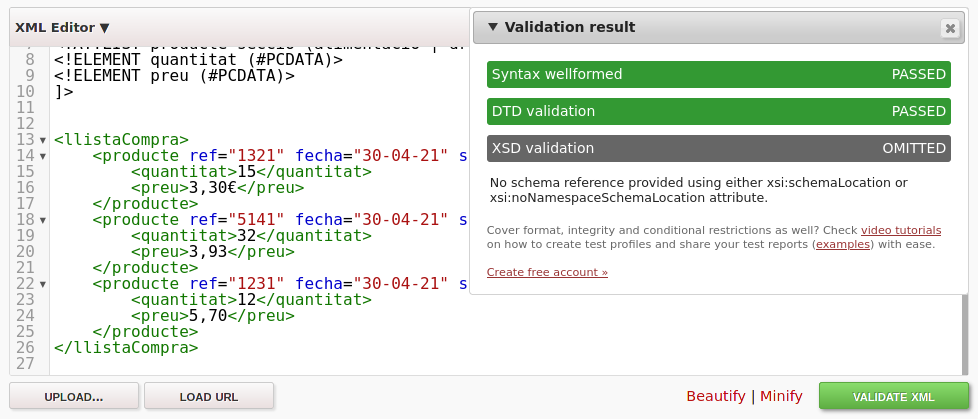
\includegraphics[width=12cm]{validacio3.png}
\end{center}

\section{Exercici 4}

\begin{verbatim}
<?xml version="1.0" encoding="UTF-8"?>

<!DOCTYPE seccio_esportiva [
 <!ELEMENT seccio_esportiva (esport*)>
 <!ELEMENT esport (equip, categoria?, poblacio)>
 <!ATTLIST esport nom NMTOKENS #REQUIRED>
 <!ATTLIST esport modalitat (individual | grup) #REQUIRED>
 <!ELEMENT equip (#PCDATA)>
 <!ATTLIST equip codi ID #REQUIRED>
 <!ELEMENT categoria (#PCDATA)>
 <!ELEMENT poblacio (#PCDATA)>
 <!ATTLIST poblacio pais CDATA #IMPLIED>
 ]>
<seccio_esportiva>
    <esport nom="Atletisme" modalitat="individual">
        <equip codi = "C01">Club Els Verds</equip>
        <categoria>Categoria Important</categoria>
        <poblacio pais="Espanya">Llucmajor</poblacio>
    </esport>
    <esport nom="Bàsquet" modalitat="grup">
        <equip codi="C02">Club Els Grocs</equip>
        <categoria>Infantil Masculí</categoria>
        <poblacio>Palma</poblacio>
    </esport>
    <esport nom="Bobsleigh" modalitat="individual">
        <equip codi="C03">Bobsleigh de Randa</equip>
        <categoria>Jocs d'hivern</categoria>
        <poblacio>Algaida</poblacio>
    </esport>
</seccio_esportiva>
\end{verbatim}
\vspace{0cm}
\begin{center}
    \textit{Comprovant de validació.}
    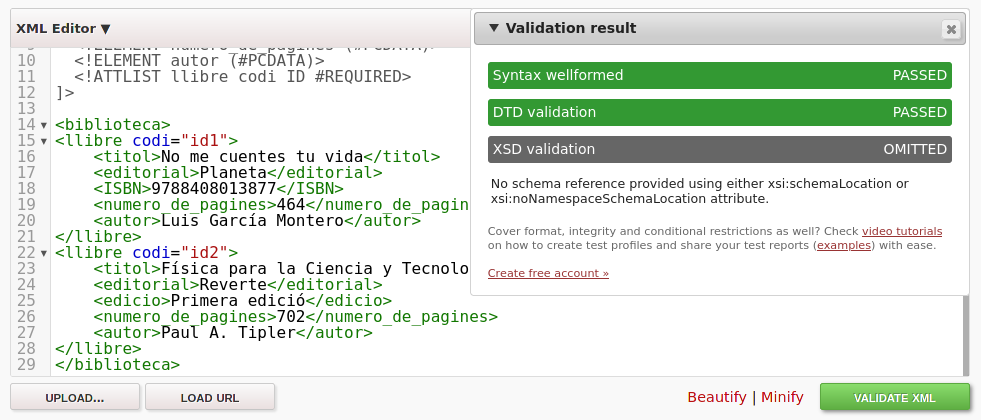
\includegraphics[width=12cm]{validacio2.png}
\end{center}
\end{document}